\begin{savequote}[75mm] 
Our posturings, our imagined self-importance, the delusion that we have some privileged position in the Universe, are challenged by this point of pale light.
\qauthor{Carl Sagan, Pale Blue Dot, 1994} 
\end{savequote}

\chapter{Visualization in Bioinformatics} \label{section:visualization}




\begin{description}
	\item[First author publications]:\\
		\begin{enumerate}
			\item \label{paper:PPI} \bibentry{SAL2014}
			\item  \label{paper:PINV} \bibentry{SAL2014pinv}
%			\item Gustavo A. Salazar et al. \emph{PPI layouts: BioJS components for the display of Protein-Protein Interactions} in  \emph{F1000Research} 2014, 3:50 (doi: 10.12688/f1000research.3-50.v1) [v1; ref status: indexed, http://f1000r.es/2u5]
%			\item Gustavo A. Salazar et al. \emph{A web-based protein interaction network visualizer} In \emph{BMC Bioinformatics} 2014, 15:129  doi:10.1186/1471-2105-15-129
		\end{enumerate}

	\item[Coauthor publications]:\\
		\begin{enumerate}
			\setcounter{enumi}{2}
			\item \label{paper:biojs1} \bibentry{GOM2013}
			\item \label{paper:biojs2} \bibentry{COR2014}
%			\item John Gomez et al. \emph{BioJS: an open source JavaScript framework for biological data visualization} in  \emph{Bioinformatics}  2013 29 (8): 1103-1104. doi: 10.1093/bioinformatics/btt100
%			\item Manuel Corpas et al. \emph{BioJS: an open source standard for biological visualisation – its status in 2014} In \emph{F1000Research} 2014, 3:55 (doi: 10.12688/f1000research.3-55.v1)  [v1; ref status: indexed, http://f1000r.es/2yy]
		\end{enumerate}
 
	\item[Author's Contibutions]:\\
		\begin{enumerate}
			\item Critical revision of the manuscript for important intellectual input: GS, AM and NM. Supervision: NM. Study concept: GS, AM and NM. Software development: GS. Drafting of the manuscript: GS and AM. All authors have read and approved the final manuscript.
			\item Critical revision of the manuscript for important intellectual input: GS, AM, GM, HR, RA and NM. Study concept: GS, AM and NM. Software Design: GS, AM, GM, HR, RA and NM. Software development: GS and AM. Creation of datasets: GM, HR and RA. Software Testing: GM, HR, RA and NM. Software Documentation: GS and RA. Drafting of the manuscript: GS, HR and NM. Supervision: NM. All authors read and approved the final manuscript;
			\item All authors have participated in the development of the BioJS community through provision of code, meeting attendance or writing of grants.
			\item All authors have participated in the development of the BioJS community through provision of code, meeting attendance or writing of grants.
		\end{enumerate}
\end{description}
\newpage
\newthought{A single point in a photograph can represent our whole known world}, as shown in the famous image acquired by the Voyager 1 spacecraft in 1990. From that perspective, is impossible to perceive all details that conform our planet, from rivers to highways, from mountains to buildings, even countries or full continents and oceans are undistinguished in the mentioned picture. Nonetheless, the image gave us a insight of the vastness of the universe in comparison with our known world.

As in the previous example the same object can be seen from different perspectives. Each of them can highlight some features and hide others, hence the importance of choosing the right representation for the object in display.

This chapter describes the contributions that are the object of this PhD project on the visualisation of bioinformatics data. We first described BioJS, a community project to create a library of bioinformatics web component, including a set of components that have been developed to be part of the library. The second part of this chapter focuses on PINV, a tool to visualise PPI networks using web technologies.


\section{BioJS: A JavaScript framework for Biological Web 2.0 Applications }
We participated in the community effort to create an specification and develop an standard for web components in Javascript, called BioJavaScript, or BioJS for short. BioJS has been described in the publications \ref{paper:biojs1} and \ref{paper:biojs2} listed at the beginning of this chapter. We believe relevant to include a description about BioJS, not only because of our contribution to it, but also because we have followed the proposed standard for the creation of a set of visualisation components described in the section \ref{subsec:biojs_components}. Some of those components were used to create the web based tool PINV, described in section \ref{section:pinv}.

BioJS is an open-source and community-driven project that aims to provide a framework to facilitate the reutilisation of JavaScript components for the visualisation of biological data in the web \cite{GOM2013}. At the hearth of the project is a registry of components (\url{http://www.ebi.ac.uk/}) in which developers following the BioJS guidelines can publish their components; and simultaneously creators of web content for biological tools, can find the right visualisation widget for their purposes.

The project started at the EBI in 2011 and its first version was officially released when the first publication about the project was written \cite{GOM2013}. By then, the registry had 29 component registered, thanks to an effort from all the collaborators in order to count with a heterogeneous set of components for this release.

In the first version a BioJS component should followed the object oriented paradigm and inherit from a common class called BioJS. In this class certain routines were implemented in order to ensure a common behaviour in between the components. The most important things included in this class were: an event manager, an object creation subroutine, an standard way to receive parameters and group of utility functions.

Because of this simplicity, BioJS components are flexible enough to manipulate the adequate web elements for visualisations: SVG, Canvas, CSS, and in general anything that can be controlled via Javascript. BioJS is framework agnostic, allowing each component to define its own dependencies. This schema supports the interaction through of two or more components that have been implemented using different JavaScript frameworks (e.g. JQuery, YUI, Prototype, etc.).
 
Another aspect defined in BioJS was the use of JSDoc format and tool to include in-code comments, this code was not only use to create the usual reference documentation, but it was key in the generation of the running examples of the components in the registry. 

In BioJS 1.0 the developer was requested to include as part of the documentation snippets of its code and a list of the dependencies and its locations.That information is use to generate the pages in the registry that include a running example, instructions on how to include the dependencies, and all the generated documentation for methods, events and parameters.

\begin{figure}  
\centering
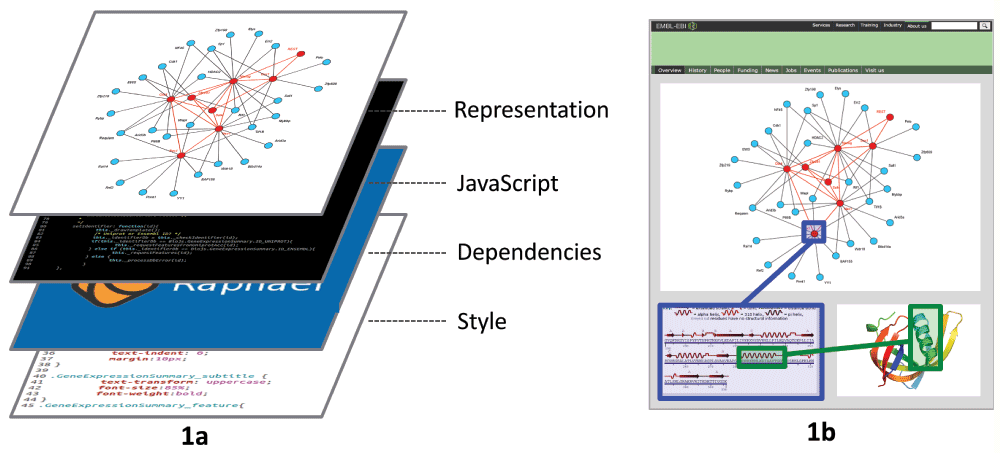
\includegraphics[width=\textwidth]{figures/biojs_layers.png}
\caption[BioJS layers.]{1a shows the different layers that a BioJS component is divided into. The representation layer sits on top of the JavaScript layer, which similarly possesses a layer of dependencies and a style. 1b presents an example of interactivity between three components, a protein-protein interaction network viewer, a secondary structure viewer and a tertiary structure viewer. Proteins in the network are represented as nodes and their interactions as edges. Clicking on a node makes the secondary and tertiary structure viewers retrieve the same protein. It is possible to select a secondary structure element in the 2D viewer and see where it is located in the 3D visualisation component.
\label{fig:biojs_layers}}
\end{figure}
 
Figure \ref{fig:biojs_layers} has in its left the layer separation in the BioJS architecture. The final representation of a component can be deployed in any of the different methods supported in web, the control of such representation is programmed in JavaScript, supported by any of the libraries the developer choose to have as dependencies. If the chosen representation is based on HTML standards, all its elements can be stylised via Cascade Style Sheets CSS \cite{COR2014}.

Here are some examples of different methods to represent data in web with examples of BioJS components using them.
\begin{description}
\setlength\itemsep{-0.3em}
\item[HTML documents] Where HTML is generated to display data, for instance \emph{Biojs.InteractionsTable} (\url{http://www.ebi.ac.uk/Tools/biojs/registry/Biojs.InteractionsTable.html}) creates a HTML table that contains information about protein interactions (Figure \ref{fig:biojs_components} a).
\item[Visualizations using HTML elements] Similar to the previous one, but the HTML generated is organise in certain way to represent the data. For example,  \emph{Biojs.Chromosome} (\url{http://www.ebi.ac.uk/Tools/biojs/registry/Biojs.Chromosome.html}) uses the div HTML element to create boxes representing the bands of a chromosome (Figure \ref{fig:biojs_components} b).
\item[Scalable Vector Graphics] HTML supports the SVG format, and because SVG is a Markup language, its manipulation is similar to when dealing with HTML content. The \emph{Biojs.FeatureViewer} (\url{http://www.ebi.ac.uk/Tools/biojs/registry/Biojs.FeatureViewer.html}) uses this technique to display protein annotations (Figure \ref{fig:biojs_components} c).
\item[HTML canvas] Since HTML5 the element canvas is part of the specification, this component provides programatic what to generate graphics. It is faster than SVG, but doesn't offer as much control on each of the drawn elements. For example, a representation of the metabolic pathways provided by KEGG is displayed by the \emph{Biojs.KEGGViewer} (\url{http://www.ebi.ac.uk/Tools/biojs/registry/Biojs.KEGGViewer.html}) component using the canvas element (Figure \ref{fig:biojs_components} d).
\item[Browser plugins] The use of third party methods such as Java Applets or Adobe Flash objects is also possible as long an interface with JavaScript is provided, for example \emph{Biojs.Protein3D} (\url{http://www.ebi.ac.uk/Tools/biojs/registry/Biojs.Protein3D.html}) displays the 3D structure of a proteins by using the JMol Java applet (Figure \ref{fig:biojs_components} e).
\end{description}

Besides the diversity in the underlined technology choose to represent the data, figure \ref{fig:biojs_components} also shows the variety of visualisation techniques that can be implemented using BioJS, from text tables to 3D objects.

\begin{figure}  
\centering
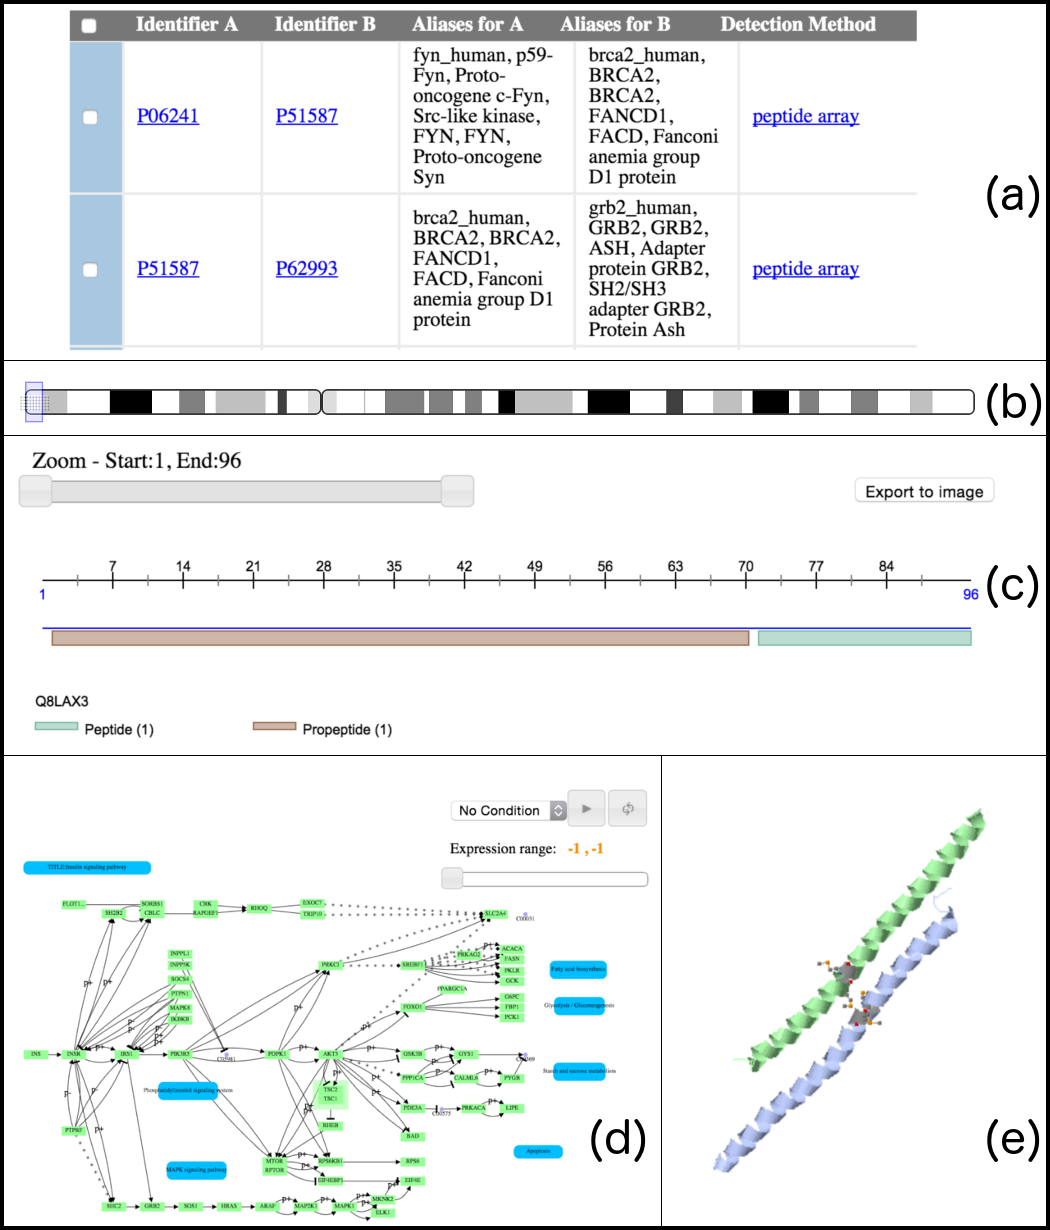
\includegraphics[width=\textwidth]{figures/biojs_components.png}
\caption[Snapshots of some BioJS components.]{Snapshots of some BioJS components. (a) Biojs.InteractionsTable, (b) Biojs.Chromosome, (c) Biojs.FeatureViewer, (d) Biojs.KEGGViewer and  (e) Biojs.Protein3D.
\label{fig:biojs_components}}
\end{figure}
 


BioJS ambitious vision is ``\emph{that every online biological dataset in the world should be visualised with BioJS tools}''. In order to accomplish it, BioJS requires to provide a convenient environment for the different roles related to the visualisation of biological data. The roles that we have identified are: data providers,  developers of web components, developers using ready-to-use components and the users that finally visit web tools that include those components.

A data provider can benefit from BioJS by simply reusing existing components that can visualise their type of data, and in this way save the resources that a development form scratch requires. Even if there is not component that fully covers the needs of the institution, is likely that there is a component that provide a partial solution, and thanks that BioJS an open-source project, the institution can extend the existing component, improving its feature set, or create an alternative version of it tailored to the needs of the institution. In the case where the required representation is so unique, that the institution requires to develop the component from scratch, they still get the benefit of ensuring that anyone else who will display their data, will count with a widget that visualise it exactly in the way they intended to do so. The two last cases ultimately reflect in growth over the BioJS library for the benefit of other BioJS actors.

Developers creating new visualisations with BioJS can get exposure and acknowledgements for their efforts. Their widgets will be now visible in an open forum, where a community of potential users and collaborators can both, benefit and contribute to the improvement of the widget. On the technical side, a developer following the BioJS guidelines is not limited by any dependency, and although the need of writing documentation and apply a code structure implies more time on the creation of the resource, it also ensures the robustness of the components.

When a developer wants to include a component to display some type of biological data, they can take advantage of BioJS by easily follow the common installation instructions provided in the registry, which have been customised for each of the components. The registry supports navigation and search of components, but we consider the bigger benefit for developers is to be able to show live demos of the components and the code to generate them. In this way, someone interested in a widget can seen it in action, without having to install or develop anything.

All of it has as final beneficiary the researcher, who ultimately is the one who will interact with the different components getting a dynamic view of the data in the way the provider expected, in a component that can be improved by a community of visualisation experts, and has been chosen to be in the web tool that the user is visiting because it is the one that highlights the features of the data in the best way.

We are aware that this is still a work in progress, but the results so far obtained from the project are very positive. For example, the journal F1000research decided to publish an special collection of articles describing BioJS component. We discussed before our opinion about how positive is for projects to provide an environment for the publication of peer-reviwed articles (Section \ref{subsubsec:ppi_biojs}). We consider the existence of this collection of BioJS projects is an important step in the right path for the growth of the project and its contributions to the research community. The section \ref{subsubsec:ppi_biojs} describes the details of an article included in this collection, in which BioJS components for the visualisation of PPI networks are explained.

\subsection{BioJS 2.0}
Besides the relative success of the first version of BioJS, its community identified a number of deficiencies and areas where the project can be improved. For example after the first version of the core was released, the focus of the community was directed to new components, and for around 3 years the code did not change much. During that time some of the libraries and strategies used were outdated: The registry required compilation using maven(http://maven.apache.org/) in order to generate the web content for each of the components. This seemed a good idea at the beginning of the project, however became a problem because of the delay in the publication of components, and more importantly the lack of a protocol to retrieve the dependencies of each component.

The registry was still bringing visibility to the components in it, but it was failing to attract developers to create new widgets using the proposed guidelines. This was the main motivation to work on BioJS 2.0.

A concentrated effort looking to push forward the new version of BioJS was held during the 4th and 6th of August of 2014. The event was hosted in Munich Germany (\url{http://biojs.net/code/2014/07/04/announcing-hackathon.html}), but it was also possible to collaborate remotely. 

The motto of this event and smaller ones held during the last months of 2014, was to bring ``easiness'' back to BioJS. The efforts were manly made from the point of view of the developer of new components: BioJS should be easy to develop, maintain and test, which should be done without failing to offer the benefits to the other BioJS stake holders; and therefore BioJS should also be easy to use, combine and discover.

The main strategy to be able to provide the desired ``easiness'' was to give freedom to the developer, which in BioJS terms meant to deprecate the predefined class, where all the components used to inherit, it also implied to abolish the requirement to follow the JSDoc format to document and introduce working pieces of code.

The alternative was to define a set of guidelines called ``the gold standard". It includes recommendations on how to test, document, publish and create examples of the component. The registry should automatically detect the recommendations followed by a component, and present this information to user exploring the components.

This implementation in the registry was done by extensively use two well know development resources available in the web: GitHub and the node package manager (npm). All the code of BioJS was migrated to the source control system git, including core, registry and components, and the repositories are hosted by GitHub (\url{https://github.com/biojs/}).

\subsection{Developed Components} \label{subsec:biojs_components}
\subsubsection{Protein-Protein Interactions networks} \label{subsubsec:ppi_biojs}
\subsubsection{Chromosome Viewer}
\subsubsection{Other Components}

\section{PINV, a web-based Protein Interaction Network Visualiser }  \label{section:pinv}
Protein-protein interaction data has been used in multiple research scenarios: (i) to browse networks for genes of interest, (ii) to interpret the results of genome-wide genomic screen, (iii) to interpret functional genomics data and (iv) to elucidate disease genes \cite{FRA2013}. In all of them visualisation has play an important role, where is to for instance,  to meaningful navigate around a big network (i and iv), to find clusters of proteins with shared functionalities(iii and iv)  or highlight links that are not evident with other techniques (i and ii).

The web is a platform for cooperative efforts, where the roles for authors and readers, providers and consumers; are harder to distinguish.

\subsection{Architecture}
\subsection{Implementation}
\subsection{Description of the application}
%\subsection{Use Cases}

\subsection{Spacial clustering for big networks on a force-directed layout}

\section{Discussion}


